\newpage
\section{Calculo numerico}
\subsection{Polinomio de taylor}
$$f(x) \approx f(x_0) + f^{'}(x_0)(x-x_0) + \frac{f^{''}(x-x_0)^2}{2!}$$

$$= \sum\limits_{i=0}^{n} \frac{f^{i}(x_0)(x-x_0)^i } {i!} \;\;\;\;\;\;\;\;\;\;\;\;\;\;\;\;\;\;\;\;$$
\subsection{Newton Raphson}
$$ P_{n+1} = P_n - \frac{f(P_0)}{f^{'}(P_0)} $$

\subsection{complemento a uno}
se cambian 1 por ceros y viceversa
\subsection{complemento a dos}
de derecha a izquierda y apartir del primer 1 encontrado sin incluirlo se 
hace la operacion de complemento a uno
\subsection{convertir de punto flotante a decimal}
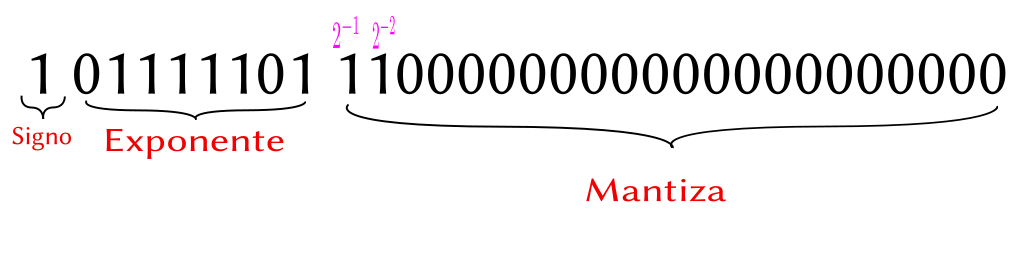
\includegraphics[scale = 0.5]{1.png}
Ejemplo:

$$(-1) \times (1+mantisa) \times {2^{expo - maxExpo} } $$
$$(-1) \times (1+0.75) \times 2^{124-127} $$
$$ = -0.21875$$

\subsection{convertir de decimal a punto flotante}
Ejemplo:
$$171.25 = 10101011,01$$

Se pasa a una forma con exponente dejando solo un entero

$$1,010101101 \times 2^7 $$

El primer bit es de signo $$1 = -$$ $$0 = +$$

Los siguientes 8 numeros son el maximo exponente mas el exponente al que esta
elevado el 2 $$127+7 = 134$$ se convierte el 134 a base 2
$$134_10 = 10000110_2$$ y la parte decimal es la mantiza, que queda igual
$$010101101$$

\newpage
\subsection{Convertir de decimal fraccionario a punto flotante}
para convertir de fraccionario a binario primero se convierte la parte entera y la parte fraccionaria se convierte usando el siguiente codigo

Codigo:

\begin{minted}{c}
	//se da un flotante de la forma 0.321312 con 
	//el numero de digitos a convertir
	//ejemplo
	//in: 0.42344 3
	//out: .001
	string FraccionBinaria(float FraccionDecimal,int NumeroDeDigitos)
	{
		string ans = ".";
		for(int i=0;i<NumeroDeDigitos;i++)
		{
			FraccionDecimal*=2;
			if(FraccionDecimal > 1.0)
			{
				FraccionDecimal-=1.0;
				ans.push_back('1');
			}
			else
			{
				ans.push_back('0');
			}
		}
		return ans;
	}
\end{minted}

\subsection{Punto Fijo}
de una ecuacion se despeja x y se substituye, tomando el resultado anterior
empezando desde una x arbitraria
\subsection{Diferencias Divididas}
$$f[x_0,x_1] = \frac{f(x_1)-f(x_0)}{x_1-x_0}$$
$$f[x_0,x_1,x_2] = \frac{f(x_1,x_2)-f(x_0,x_1)}{x_2-x_0}$$
$$ f[x_0,x_1,x_2,x_3] = \frac{x_2,x_3) - f(x_0,x_1)}{x_3-x_0}$$
$$P_n = a_0 + a_1(x-x_0) + a_2(x-x_0)(x-x_1) + ... + a_n(x-x_0) \times ... \times (x-x_n)$$

\begin{center}
 \begin{tabular}{|c c c c c|} 
 \hline
	 $j$ & $X_j$ & $f(X_j)$ & 1 & 2  \\ [0.5ex] 
 \hline\hline
	 0 & $X_0$ & $f(X_0)$ & 1 &  1 \\
 \hline
	 1 & $X_1$ & $f(X_1)$ & $f(X_0,X_1)$ & 1 \\
 \hline
	 2 & $X_2$ & $f(X_2)$ & $f(X_1,X_2)$ & $f(X_0,X_1,X_2)$ \\
 \hline
\end{tabular}
\end{center}
\subsection{Polinomio de lagrange}
$$P_n(x) = \sum_{i=0}^{n} L_i(x)f(x_i)$$

$$
L_i(x) = \prod_{\substack{j=0 \\
	j \neq i}}^{n}
	\frac{(x-x_j)}{(x_i-x_j)}
$$



